\section{Livello 5: Application}
    \subsection{TFTP e FTP}
        Il protocllo \textbf{FTP (File Trasnfert Protocol)} è stato sviluppato per il trasferimento affidabile ed efficiente dei dati, per questo motivo si basa su TCP. Il server FTP offre anche un servizio di autenticazione per l'accesso al file-system, la gestione delle directory e dei file.
    
        FTP utilizza due porte: la TCP/21 per i comandi e la TCP/20 per i dati.
    
        Le modalità di funzionamento sono due: attiva e passiva.

        Nella modalità attiva, il client apre il canale comandi verso il server (porta 21 del server, porta random $N$ del client), mentre per la trasmissione dati il client svolge la funzione di server, ovvero rimane in ascolto sulla porta $N + 1$, mentre è il server ad iniziare la comunicazione utilizzando la porta 20.

        Nella modalità passiva, è anche compito del client dare il via alla connessione per il trasferimento dei dati.

        Il protocollo \textbf{TFTP (Trivial FTP)} è la versione semplificata di FTP, che non supporta l'autenticazione ed utilizza UDP, con il server in ascolto sulla porta 69.

        Questo significa che la gestione del flusso (numerazione dei pacchetti, Acknowledgment, gestione degli errori), viene realizzata a livello applicativo, all'interno di TFTP.

        In TFTP ogni trasferimento inzia con una richiesta di read (GET) o write (PUT).

        GET: il server risponde con un file frammentato in datagrammi numerati; ogni datagramma deve essere riscontrato.

        Il block-size di default è di 512 byte.

        Un pacchetto di dimensione inferiore, rappresenta l'ultimo pacchetto trasmesso (se la dimensione del file trasferito è un multiplo esatto della dimensione dei blocchi, il server invia un ultimo pacchetto di dati contenente 0 byte di dati).

        \begin{center}
            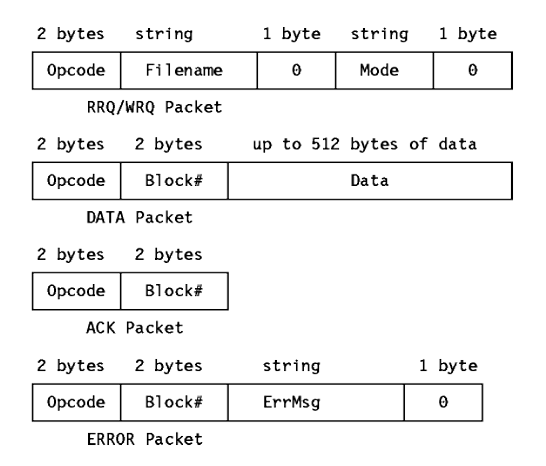
\includegraphics[scale=0.4]{chapters/6/assets/schema_a.png}
        \end{center}

        \subsubsection{Le fasi di una connessione TFTP}
            \begin{enumerate}
                \item Il client contatta il server inviando un pacchetto di tipo \textbf{RRQ (Read Request)} o \textbf{WRQ (Write Request)}.
                \item Il server risponde inviando/ricevendo pacchetti \textbf{DATA} di 512 byte.
                \item Per ogni pacchetto DATA ricevuto o inviato, viene inviato o ricevuto un \textbf{ACK} o un \textbf{ERROR}.
                \item I pacchetti vengono trasferiti finché la loro lunghezza non è inferiore a 512 byte.
                \item Termina la connessione.
            \end{enumerate}

            \begin{center}
                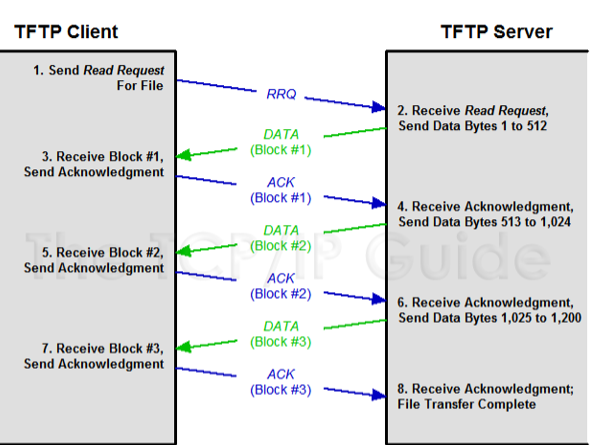
\includegraphics[scale=0.]{chapters/6/assets/schema_b.png}
            \end{center}

    \subsection{DNS}
        Lo scopo del sistema \textbf{DNS (Domain Name System)} è quello di gestire uno spazio univoco dei nomi per i nodi della rete, fornendo agli utente di IP un servizio per la traduzione nome-numero e numero-nome.
    
        Lo spazio dei nomi è strutturato in modo gerarchico, come il file-system, ma la radice è a destra (\verb:netlab.fis.unipr.it:). Il primo elemento è il nome locale del nodo, mentre gli elementi successivi (domini), seprata da un ”.”, rappresentano il percorso nella gerarchia. Un nome completo termina sempre con un punto, che rappresenta la radice della gerarchia.
        Il dominio più a destra è detto \textbf{TLD (Top Level Domain)}.
    
        I TLD sono gestiti dall'organismo internazionale ICANN (attraverso IANA) che li assegna alle organizzazioni che ne fanno richiesta, mentre i livelli successivi sono gestiti in modo autonomo dalle organizzazioni assegnatarie.
    
        Inizialmente Internet era composta unicamente dai nodi US, per cui esistono alcuni TLD che rispecchiano la struttura Statunitense originale: gov (governo federale US), com (commerciale), edu (istituzioni educative), provider di rete, org (organizzazioni-no-profit).
    
        Successivamente, con la diffusione di Internet, sono nati i TLD geografici: it, es, fr, de, etc.

        A partite dal 2000, ICANN ha approvato nuovi TLD generici quali: biz (business), info (informazioni), name (nome di persona), pro (professionali), coop (cooperative), travel (viaggi), museum (muesei), aero (aerotrasporti).

        Attualmente sono attivi i seguenti TLD:
        
        \begin{center}
            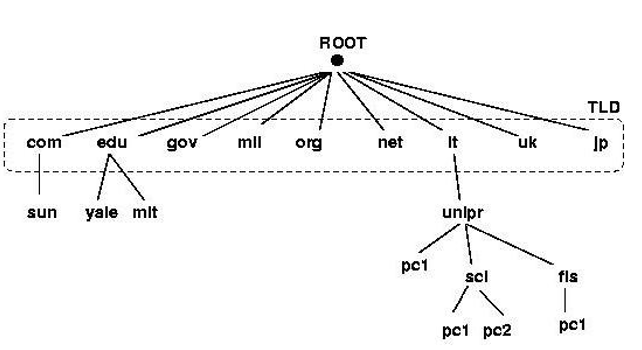
\includegraphics[scale=0.45]{chapters/6/assets/schema_c.png}
        \end{center}

        La \textbf{risoluzione inversa} consiste nella risoluzione del nome a partire dall'indirizzo IP.

        Viene usata per produrre un output leggibile nei file di log, oppure per controlli di autenticazione (es: richiedere che il client sia registrato).

        Il nome dei domini di reverse è composto dai numeri della rete (in ordine rovesciato) seguita dalla stringa \verb:in-addr.arpa:.

        Il rovesciamento del numero consiste nel ricercare i numeri nello stesso albero dei nomi, utilizzando lo stesso procedimento di parsing da destra verso sinistra.

        Ogni client deve essere configurato con l'indicazione di almeno un \textbf{server DNS locale} a cui rivolgersi per le risoluzioni,

        Il server DNS locale recupera l'informazione, interagendo eventualmente con gli altri server DNS, e la comunica al client.

        Nei sistemi Linux questa configurazione viene stabilita all'interno del file \verb:/etc/resolv.conf:. La configurazione del DNS può essere impostata dinamicamente dal protocollo DHCP assieme alle altre informazioni di configurazione (indirizzo IP, Gateway, netmask, etc.).

        I client del DNS sono generalmente i programmi applicativi che, mediante funzioni come \verb:gethostbyname():, recuperano l'indirizzo dell'host prima di contattarlo.

        Esistono anche client a linea di comando come: \verb:nslookup: e \verb:dig:.

        I TLD possono organizzarsi in sottodomini di livello 2, i quali a loro volta possono gestire domini di livello 3, e così via.

        Lo spazio dei nomi, è gestito in modo distribuito suddividendolo in \textbf{zone}. Ogni \textit{zone} include una porzione dell'albero che gestisce in modo autonomo con DNS server primario ed uno o più DNS server secondari, che ne replicano i dati (per sicurezza e prestazioni).

        Una zone si forma attraverso l'assegnazione della delega da parte del server della zone superiore, mediante il record NS.

        Ogni host è inserito in due punti dell'albero: nella zona diretta e nella zona inversa.

        \textbf{BIND} è il nome del più comune daemon DNS usato nei sistemi Unix.

        Un sever può essere configurato per diversi tipi di funzionamento:
        \begin{itemize}
            \item \textbf{Server Autoritativo di Primary Zone (Master)}.
            \item \textbf{Server Autoritativo di Secondary Zone (Slave)}.
            
            L'amministratore di zone aggiorna i dati sul Primary (su un file locale), il Primary replica i dati della zone verso i Secondary ("Zone Transfert", 53/TCP); risponde alle query che riceve (53/UDP).
            Un server autoritativo `e generalmente anche Caching NS.
            \item \textbf{Caching Name Server} (forwarder: riceve query dai client (53/UDP), ottiene la risposta interrogando i server autoritativi, mantiene copia locale in cache delle risposte ottenute, invia la risposta al client.
        \end{itemize}

        Se il server che riceve la richiesta è autoritativo per il dato richiesto, risponde direttatemente, altrimenti occorre attraversare l'albero, passando attraverso i server autoritativi coinvolti. L'attraversamento può essere ricorsivo o iterativo.

        \textbf{Modalità ricorsiva}: se il server interrogato non è autoritativo per il dato richiesto, passa la richiesta al server successivo e così via in modo ricorsivo.

        \textbf{Modalità iterativa}: il server restituisce al client l'indirizzo del server successivo. In questo modo, è il DNS locale che contatta direttamente i server coinvolti.

        Generalmente, un server ammette query ricorsive solo per i client locali.

        Internet posside 13 \textbf{Root Server} che contengono le informazioni riguardo i domini di primo livello. Questi server vengono contattati ogni volta che un client chiede informazioni relative ad altri TLD, quindi ogni DNS Resolver deve possedere una lista aggiornata dei \textit{Root Server} (file named.ca di BIND).

        I Root Server (RS) sono non-ricorsivi, ovvero se non hanno la risposta, forniscono l'indirizzo del server del TLD coinvolto.

        Le informazioni relative alla zone vengono memorizzate come \textbf{RR (Resource Record)}.

        Il formato generico di un RR corrisponde ai seguenti campi:
        \begin{itemize}
            \item \textbf{Nome}: il nome di dominio a cui questo RR si riferisce.
            \item \textbf{TTL}: tempo di vita del RR nella cache del sever DNS prima di essere eliminato.
            \item \textbf{Classe}: indentifica la famiglia del protocollo. \textbf{IN} indica il sistema Internet.
            \item \textbf{Tipo}: il tipo di RR. I tipi principali sono:
            \begin{itemize}
                \item \textbf{A}: Indica l'indirizzo IPv4 per il nome specificato.
                \item \textbf{AAAA}: Indica l'indirizzo IPv6 associato al nome.
                \item \textbf{CNAME}: Record Canonical Name, usato per indicare il nome dell'alias.
                \item \textbf{MX}: Mail eXchanger, indica un host che gestisce la posta per il dominio.
                \item \textbf{NS}: Un server DNS per il dominio specificato.
                \item \textbf{PTR}: Usato nella risoluzione inversa per associare un indirizzo IP al
                nome.
                \item \textbf{SOA}: Start Of Autority, un RR che indica il server DNS dove risiedono i dati autoritativi per questo dominio ed alcuni dati amministrativi.
            \end{itemize}
        \end{itemize}

        \subsubsection{DNS e Posta Elettronica}
            Per ogni dominio che è in grado di ricevere posta, il DNS è in grado di fornire una lista di server SMTP a cui inviare il messaggio.
        
            In questo modo, se il mail server principale del destinatario non è operativo, è possibile inviare il messaggio presso un computer di backup in grado di gestire la posta altrettanto bene.
        
            Queste informazioni sono contenute nel record MX:
            \begin{center}
                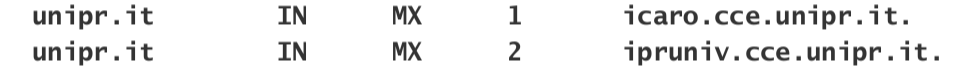
\includegraphics[scale=0.35]{chapters/6/assets/schema_d.png}
            \end{center}

            Il camppo numerico indica la priorità (il numero più basso è quello ha maggiore priorità).

        \subsubsection{Formato del pacchetto DNS}
            \begin{center}
                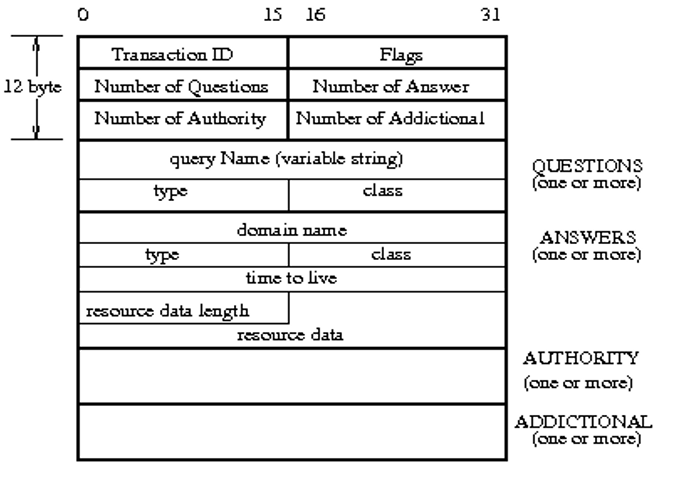
\includegraphics[scale=0.45]{chapters/6/assets/schema_e.png}
            \end{center}

            Il significato dei campi è:
            \begin{itemize}
                \item \textbf{Transaction ID}: serve per associare domanda a rispota.
                \item \textbf{Flags}: QR (domanda(0) / risposta(1)), OPCODE (4 bits, tipo di query), RD (Recursion Desidered), RA (Recursion Available); RCODE (4 bits, esito della risposta).
                \item \textbf{Question}: domanda per il DNS.
                \item \textbf{Answer}: elenco di RR che rispondono alla query.
                \item \textbf{Authority}: elenco di RR degli NS autoritativi che portano più vicini alla risposta.
                \item \textbf{Addictional}: elenco di RR con informazioni addizionali.
            \end{itemize}

            Il \textbf{dDNS (Dynamic DNS)} è una tecnologia che permette ad un nome in Internet di essere sempre associato all'indirizzo IP di uno stesso host, anche se l'indirizzo cambia nel tempo.

            Il servizio è costituito da una popolazione di client dinamici (host con indirizzo IP dinamico che vogliono che il loro IP attuale sia registrato nel DNS), da uno o più server DNS dinamici e da un protocollo di comunicazione tra le due parti.

            \verb:nsupdate: è una utility disponibile ai client per l'aggiornamento del DNS.

            I \textbf{DNSSEC (Domain Name System Security Extension)} sono una serie di specifiche dell'IETF per garantire la sicurezza e l'affidabilità delle informazioni fornite dai sistemi DNS.

            I servizi che offrono sono:
            \begin{itemize}
                \item Autenticazione: effettiva origine dei dati DNS.
                \item Integrità dei dati ricevuti.
                \item Asserzioni di non esistenza.
            \end{itemize}

    \subsection{Il protocollo Telnet}
        Il Telnet è un protocllo storico di TCP/IP creato per l'accesso remoto alla console testuale di un host. La porta assegnata da IANA è la 23/TCP.
    
        Operazioni:
        \begin{itemize}
            \item Client: il client legge lo stream dallo standard input e lo invia al server, lo stream proveniente dal server viene inviato allo standard output.
            \item Server: il server legge le linee provenienti dal client, le interpreta come comandi di console, ed invia al client l'output del comando.            
        \end{itemize}

        Telnet è un protocollo testuale (richieste e risposte sono spedite in ASCII, compresa le credenziali) ha quindi un livello di sicurezza molto basso ed è stato sostituito da protocolli più sicuri (SSH).

        Un indirizzo di posta elettronica è costituito da due identificativi: nome del server che gestisce la mailbox ed identificativo dell'utente: \verb:<utente>@<server>:, dove \verb:<server>: è l'indirizzo IP o un suo identificativo nel DNS.

        Il record MX del DNS consente di creare caselle di posta in un dominio, a cui possiamo associare uno o più server di posta per la sua gestione.

        Ogni utente ha visogno di uno \textbf{MUA (Message User Agent)} che è un programma che gli consente di inviare o leggere i messaggi della propria mailbox.

        Il MUA consegna il messaggio ad un \textbf{MTA (Message Transfer Agent)} che ha il compito di trasportare il messaggio a destinazione. Il messaggio può attraversa diversi MTA prima di arrivare nella mailbox del destinatario.

        Il primo MTA è detto anche \textbf{submission server} perché è utilizzato dai MUA per la sottomisssione delle mail e dovrebbe supportare autenticazione (SMTP AUTH).

        Sull'ultimo MTA è presente anche il \textbf{MDA (Message Delivery Agent)} che si occupa della consenga del messaggio nella mailbox dell'utente.

        Se il MUA del destiantario e il MDA sono su host diversi, occore un protocollo per la lettura dei messaggi (POP o IMAP).

        \begin{center}
            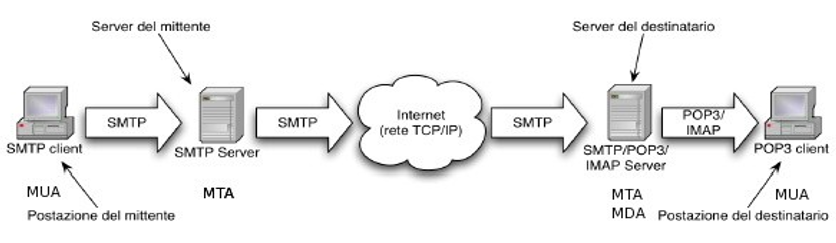
\includegraphics[scale=0.41]{chapters/6/assets/schema_f.png}
        \end{center}

        \subsubsection{Formato dei messaggi}
            Il formato dei messaggi è stato codificato nel 1982, i messaggi sono codificati in ASCII standard ed organizzati in righe di max 1000 caratteri.
        
            Il formato dei messaggi è:
            \begin{itemize}
                \item Intestazione (header)
                \item \verb:<cr> <lf>: (riga vuota)
                \item Corpo del messaggio (body)
            \end{itemize}
            
            Intestazione: in ogni riga la coppia \verb-<campo>:<valore>-, i principali campi:
            \begin{itemize}
                \item To: indirizzi dei destinatari
                \item CC: indirizzi destinatari secondari
                \item Bcc: destinatari secondari con indirizzi nascosti
                \item From: la persona che ha creato il messaggio (obbligatorio)
                \item Received: riga aggiunta da ogni MTA attraversato
                \item Date: data ed ora di invio del messaggio
                \item Subject: breve riepilogo del messaggio
                \item Message-ID: identificatore univoco del messaggio (generato automaticamente)
                \item User-Agent: client di posta utilizzato dall'utente
            \end{itemize}

            Esitono due formati principali della mailbox:
            \begin{itemize}
                \item \textbf{Mbox}: i messaggi ricevuti dall'utente sono accodati in un singolo file per ogni utente.
                
                In Unix si trova in \verb:/var/spool/mail/username:

                Ogni messaggio inizia con una linea: \verb:From sender@domain..:
                \item \textbf{Maildir}: si utilizza una directory per ogni utente, all'interno di essa viene creato un file di testo per ogni messaggio ricevuto.
            \end{itemize}

    \subsection{MIME}
        Il formato del 1982 era stato pensato solo per messaggi di testo espressi in ASCII standard.
    
        Si utilizza adesso una nuova soluzione \textbf{MIME (Multipurpose Intenet Message Extensions)} che introduce 5 nuove intestazioni:
        \begin{itemize}
            \item \textbf{Mime-version}
            \item \textbf{Content-descriptor}
            \item \textbf{Content-id}
            \item \textbf{Content-transfer-encoding}: il nome dello schema di codifica utilizzato per trasformare il messaggio in ASCII standard. I principali valori sono:
            \begin{itemize}
                \item \textbf{ASCII 7bit}: nessuna codifica; linee fino a 1000 caratteri.
                \item \textbf{ASCII 8bit}: viola la versione originale del protocollo.
                \item \textbf{Quoted-printable}: messaggi ASCII non standard: i caratteri superiori a 127 sono codificati con "=" seguito dal codice ASCII in esadecimale (es. città $\rightarrow$ citt=9A).
                \item \textbf{base64}: utilizzato per i dati binari, ogni sequenza di 6 bit viene trasformata in un carattere ASCII grazie ad una codifica di 64 simboli (sprecati 2 bit ogni 6, i dati codificati occupano il 35\% di spazio in più.
                
                Codifica: openssl \verb:base64 -e -in img.png-out img.b64:
                
                Decodifica: \verb:openssl base64 -d -in img.b64 out img.png:
            \end{itemize}
            \item \textbf{Content-type}: natura del corpo del messaggio; utile per attivare automaticamente il Viewer corretto (tipi e sottotipi sono gestiti da IANA).
        \end{itemize}

        \subsubsection{Principali Content-types}
            \begin{center}
                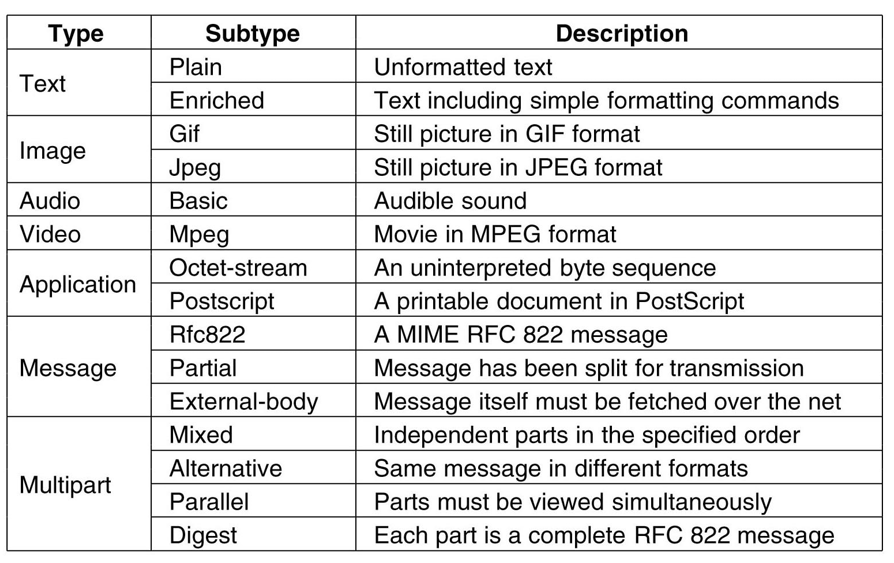
\includegraphics[scale=0.38]{chapters/6/assets/schema_g.png}
            \end{center}

    \subsection{SMTP}
        \textbf{SMTP (Simple Mail Transfer Protocol)} è un protocollo applicativo (25/TCP) che si occupa del trasferimento di un messaggio da MUA a MTA o da MTA a MTA.
    
        L'MTA può essere il destinatario finale (MTA + MDA) o di trasferimento (Mail Relay, Mail scanner, etc.).
    
        Il protocollo è codificato ASCII Standard ovvero prevede uno scambio di dati testuali.
    
        Principali comandi del client SMTP:
        \begin{itemize}
            \item HELO: indirizzi dei destinatari
            \item MAIL FROM: mittente del destinatario
            \item RCPT TO: destinatario del messaggio
            \item DATA: corpo del messaggio
            \item QUIT: fine del messaggio
            \item RSET: reset
            \item HELP: nome del comando
        \end{itemize}

        Principali risposte del server SMTP:
        \begin{itemize}
            \item 220: servizio pronto
            \item 250: comando richiesto completato
            \item 251: utente non locale, il messaggio sarà inoltrato
            \item 221: chiusura canale di trasmissione
            \item 421: servizio non disponibile
            \item 500: errore di sintassi
            \item 501: errori di sintassi nei parametri
            \item 554: transazione fallita
        \end{itemize}

        \subsubsection{MUA: Mail User Agent}
            Un MUA è una applicazione che viene usata per inviare e ricevere la posta elettronica.
        
            \verb:mail:: è il MUA di base nei sistemi Linux (non gestisce allegati MIME), è utilizzato per leggere la posta che risiede sul server MDA (non gestisce POP3 / IMAP). L'invio è affidato all'MTA su localhost.
        
            L'opzione \verb:-v: visualizza il dialogo SMTP con l'MTA.
        
            \verb:alpine:: è un MUA testuale, ma con gestione dello schermo (gestisce gli allegati MIME).
        
            Può gestire la mailbox da remoto con il protocollo IMAP.

        \subsubsection{Sottomissione dei messaggi con SMTP-AUTH}
            Poiché il protocollo SMTP non prevede autenticazione chiunque può contattare un MTA per spedire mail verso chiunque (spam). Per questo motivo spesso gli MTA accettano esclusivamente messaggi in cui il mittente o il destinatario sono locali.
        
            Inoltre le porte 25 (SMTP) sono spesso bloccate dai firewall per forzare l'utilizzo di MTA istituzionali (dotati di antivirus e antispam).
        
            Gli utenti mobili (nomadic users) però vogliono contattare il proprio mail server anche quando sono fuori sede (mittente e destinatario non locale). I server ESMTP generalmente supportano l'autenticazione con SMTP-AUTH per la fase di sottomissione di e-mail attraverso l'introduzione di un MTA dedicato denominato \textbf{MSA (Message Submission Agent)}.

            Tramite l'estensione SMTP AUTH è possibile:
            \begin{itemize}
                \item richiedere le credenziali (user/pass) del client.
                \item utilizzare tecniche crittografiche per la cifratura dei messaggi scambiati.
                \item utilizzare una porta di ascolto diversa: 587/tcp.
            \end{itemize}

            La consegna del messaggio della mailbox utente è gestita dall'\textbf{MDA (Message Delivery Agent)} che ha anche il compito di consegnare il messaggio al MUA dell'utente previo opportuno meccanismo di autenticazione.

            Quando è nato il protocollo SMTP gli utenti lavoravano sulla stessa macchina dove risiedevano le Mailbox, che quindi il MUA poteva accedere direttamente. Con l'avvento dei PC il MUA si è disaccoppiato dall’MDA ed è nata la necessità di nuovo protocollo di rete per la comunicazione MUA-MDA.\\
            Due possibili protocolli: POP3 o IMAP.

        \subsubsection{POP3}
            \textbf{POP3 (Post Office Protocol 3)} è un protocllo ASCII con autenticazione per il trasferimento dei messaggi dal mailbox allo user agent utilizzando un servizio TCP sulla porta 110.
        
            Dopo la connessione il protocollo attraversa 3 fasi:
            \begin{itemize}
                \item Autenticazione: invio delle credenziali (USER e PASS)
                \item Transazioni: Esecuzione dei comandi (LIST, RETR, DELE, QUIT)
                \item Aggiornamento: Dopo il QUIT il server cancella effettivamente i messaggi eliminati e interrompe la connessione                
            \end{itemize}

            POP3 è utilizzato tipicamente da Home Users, connessi via modem o ADSL all'ISP, per trasferire (RETR) tutti i nuovi messaggi, che vengono poi eventualmente cancellati dal server (DELE). Il mailbox server funziona così da area di transito per i messaggi, che vengono gestiti sull'hard disk dell'utente.

        \subsubsection{IMAP}
            \textbf{IMAP (Internet Message Access Protocol)}, è un protocollo alternativo a POP3 per consentire all'user agent la gestione dei messaggi ricevuti, utilizzando il servizio TCP sulla porta 143.
        
            A differenza di POP3 presume che i messaggi debbano rimanere sul server. Per questo fornisce la possibilità di gestire cartelle di posta sul server in cui archiviare i messaggi ricevuti.
        
            IMAP è adatto per utenti che accedono alla posta utilizzando diversi user agent (casa, lavoro, portatile, etc.).

    \subsection{World Wide Web}
        \textbf{WWW (Word Wide Web)} è un'architettura client/server per la consultazione in rete di documenti multimediali ed ipertestuali distribuiti in rete.

        L'architettura è nata nel 1989 al CERN di Ginevra e dal 1994 il suo sviluppo è gestito dal consorzio \textbf{W3C} (accordo CERN-MIT).

        \textbf{HTML (HyperText Markup Language)} è il formato con cui vengono descritti gli ipertesti.

        \textbf{HTTP (HyperText Transfer Protocol)} è il protocollo principale per la comunicazione tra client e server, anche se l'architettura WWW consente l'utilizzo di protocolli diversi.

        Ogni documento WWW o singolo oggetto multimediale (file audio, immagine, etc.) è identificato mediante un indirizzo univoco in Internet (URL) e può contenere riferimenti ipertestuali ad altri documenti.

        I documenti possono essere statici (già presenti sul server al momento della richiesta) o dinamici (generati al momento della richiesta dal server o dal client). L'utente accede ai documenti fornendo l'URL al programma client (Web Browser).

        \begin{center}
            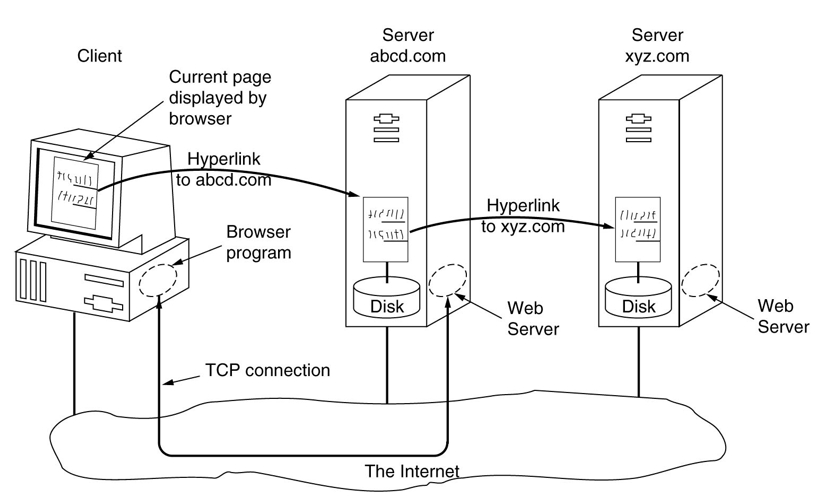
\includegraphics[scale=0.4]{chapters/6/assets/schema_h.png}
        \end{center}

        \subsubsection{URL}
            Gli \textbf{URL (Uniform Resource Locator)}, sono identificatori univoci di documenti WWW.

            Sono composti da 4 parti:
            \begin{itemize}
                \item \textbf{Schema}: è il protocollo per raggiungere il dominio.
                \item \textbf{NomeServer}: è il nome DNS del server che contiene il documento.
                \item \textbf{Port}: è la porta di ascolto del server.
                \item \textbf{NomeLocale}: è l'identificatore del documento sul server.
            \end{itemize}

            HTTP è il protocollo più utilizzato per l'accesso ai documenti WWW, altri schemi diffusi sono ftp, file, about.

        \subsubsection{Tipi MIME}
            Oltre ai documenti ipertestuali HTML l'architettura WWW supporta un numero sempre crescente di altri formati.
        
            Per alcuni formati il browser conterrà l'interprete necessario per visualizzarli, per altri formati si appoggerà a componenti software esterne, i \textbf{plug-in} o gli \textbf{helper}.
        
            Un plug-in è un modulo esterno che il browser installa come estensione di se stesso.
        
            L'helper (o applicazione di supporto) è un programma autonomo eseguito come processo separato a cui il browser passa il file da visualizzare.
        
            Per ogni MIME-Type il browser avrà associata la modalità di gestione utilizzando uno dei metodi precedenti. In alcuni casi il documento viene aperto da un file locale, senza il MIME-Type fornito dal server. In questi casi l'associazione si basa sull'estensione del file.

        \subsubsection{I Web Browser}
            I \textbf{web browser} sono applicazioni client di WWW; sono prevalentemente grafici (Firefox, Chrome, etc.) ma anche testuali (lynx).
        
            Dispongono di una cache su disco per i documenti visitati di recente. Sequenza di operazioni del client:
            \begin{itemize}
                \item Input dell'URL.
                \item Verifica se il documento è presente in cache.
                \item Risoluzione del nome DNS nell'indirizzo IP.
                \item Invio della richiesta al server mediante il protocollo indicato nello schema.
                \item Ricezione del documento inviato dal server.
                \item Parsing del documento.
                \item Eventuale richiesta di documenti collegati.
                \item Visualizzazione del documento direttamente o mediante viewer esterni.
                \item Rilascio della connessione TCP (se non vi sono altre richieste entro breve termine).
            \end{itemize}
        
        \subsubsection{I Web Server}
            Il \textbf{web server} è un programma che si occupa di fornire, su richiesta del client browser, una pagina WWW.
        
            \textbf{The Apache Software Foundation} è il nome di un gruppo di lavoro che sta portando avanti diversi progetti Open Source tra cui i più diffusi Web Server: \textbf{Apache} e \textbf{Tomcat}.
        
            Sequenza di operazioni del server:
            \begin{itemize}
                \item Accetta la connessione TCP da un client.
                \item Determina dall'URL il percorso del documento richiesto.
                \item Accede al documento sul disco.
                \item Invia al client di intestazione (Mime-Type).
                \item Rilascio della connessione TCP.
            \end{itemize}

            Un web server può essere sottoposto ad un carico elevato: parecchie richieste al secondo di documenti statici (che stanno su disco) o dinamici (vengo creati al momento della richiesta da una elaborazione).

            Per migliorare le performance del server esistono diverse strategie, quali:
            \begin{itemize}
                \item Lettura da disco lenta: implementazione di un sistema di caching.
                \item Server multithread: le richieste sono gestite da un front-end che smista la richiesta un modulo di elaborazione (thread) libero e torna in ascolto.
            \end{itemize}

            \begin{center}
                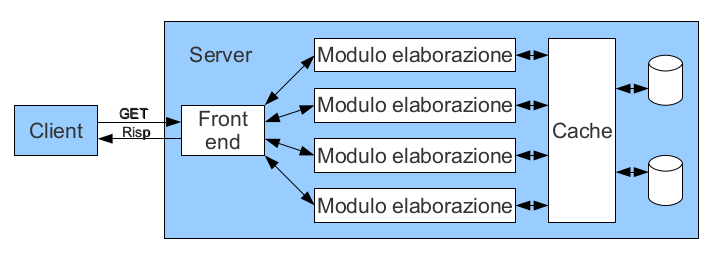
\includegraphics[scale=0.4]{chapters/6/assets/schema_i.png}
            \end{center}

        \subsubsection{Web Caching}
            Fare \textit{caching} significa memorizzare temporanemente le pagine in un punto più vicino al client per una visualizzazione più rapida e per ridurre il carico del server.
            
            I browser operano automaticamente caching sul disco locale dei documenti visitati.

            Se il documento richiesto è presente sul disco locale viene fatto un GET condizionale (if-modified-since), in cui si chiede se esiste una versione più recente del documento.

            Una LAN può organizzare un servizio di caching disponibile per tutti gli utenti della rete.\\
            Per utilizzare il servizio, l'utente deve attivarlo esplicitamente. Questo servizio di cache viene denominato \textbf{proxy} poiché l'accesso al server che contiene il documento richiesto viene realizzato da \textbf{proxy/cache} server.\\
            Questo meccanismo consente l'accesso ai server Web in Internet anche da parte di client Intranet della LAN (configurati con un indirizzo IP privato).
        
            \begin{center}
                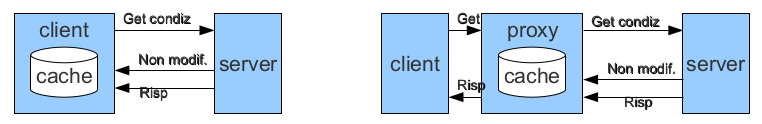
\includegraphics[scale=0.4]{chapters/6/assets/schema_j.png}
            \end{center}

        \subsubsection{Content Delivery Network (CDN)}
            Per contenuti che devono essere distribuiti su scala globale (downloads, streaming, etc.) esistono due approcci: \textbf{web caching} e \textbf{CDN}.

            Con il web caching è il client ad attivare le copie, mentre con CDN è il provider che distribuisce copie dei contenuti in un insieme di nodi in differenti posizioni ed istruisce i client in modo che usino un nodo a lui vicino.

            Possibili architetture per realizzare una rete CDN:
            \begin{itemize}
                \item \textbf{DNS redirection}: il name server della CDN è gestito dalla CDN stessa. Il client ottiene dal DNS l'indirizzo Unicast della copia più vicina a lui.
                \item \textbf{Routing Anycast}: i mirror server hanno gli stessi indirizzi Anycast e il compito di trovare il server più vicino è demandato al routing anycast.
            \end{itemize}

            Una delle reti CDN più note è Akamai, con oltre 29'000 server sparsi su circa 70 nazioni.

        \subsubsection{Expiration}
            Alcuni documenti HTML possono contenere un'intestazione Expires che indica il tempo di validità del documento e verrà utilizzata per decidere se utilizzare la copia o recuperare il documento dal server.

            \lstinputlisting[language=HTML]{chapters/6/assets/schema_k.html}

            Altri documenti usano l'intestazione "no-cache" per impedire che il documento venga inserito nella cache (tipicamente pagine dinamiche).

            \lstinputlisting[language=HTML]{chapters/6/assets/schema_l.html}

        \subsubsection{HTML}
            La maggior parte dei documenti WWW sono scritti in HTML.
        
            HTML è un linguaggio di markup, ovvero contiene direttive di formattazione. I contenuti sono testo formattato (font, colore, liste, tabelle, etc.) ed eventuali riferimenti ad oggetti esterni (immagini, video, suoni, hyper-link ad altri documenti).

            Le direttive per la formattazione sono dette \textbf{tag} e sono racchiuse tra parentesi angolari: (esempio \verb:<b>: testo evidenziato \verb:</b>:)

            Il documento HTML è delimitato dal tag \verb:<html>....</html>: e comprende una intestazione \verb:<head>...</head>: ed un corpo \verb:<body>...</body>:.

            HTML è uno standard in continua evoluzione:
            \begin{itemize}
                \item \textbf{HTML 2.0}: è il primo vero standard HTML, rilasciato nel 1995 da W3C.
                \item \textbf{HTML 3.2}: rilascato nel 1997, è stato adottato in diversi browser.
                \item \textbf{HTML 4.01}: rilascato nel 1999 da W3C, è un'altra release con molte implementazioni.
                \item \textbf{HTML 5}: rilasciato nel 2014 da W3C.
            \end{itemize}

            I browser e server web hanno generalmente implementato le varie release HTML in modo più o meno rigoroso, sorvolando spesso su errori di formattazione e in alcuni casi, aggiungendo tag non standard, funzionanti solo su alcune piattaforme.

            \textbf{XHTML} è un linguaggio di markup che associa alcune proprietà dell'XML nell'HTML.

            Un file XHTML è un pagina HTML scritta in conformità con lo standard XML. Per arginare questa dispersione W3C ha creato un \textbf{validatore on-line} che aiuta a scrivere documenti HTML aderenti agli standard ufficiali.

        \subsubsection{Style sheet}
            HTML è un linguaggio di markup che mescola il documento alla formattazione, infatti alcuni tag descrivono il contenuto del documento, indipendentemente dalla sua rappresentazione finale (esempio \verb:<img src=..>: oppure \verb:<a href=..>:) , mentre altri tag descrivono il modo, in cui il documento dovrà apparire al lettore (esempio \verb:<font color="red", face="arial">:).

            Con la crescente complessità e varietà di utilizzo dei documenti web, è sorta la necessità di separare i due aspetti del documento. Per questo motivo sono stati introdotti i \textbf{fogli di stile (style sheet)} che sono file associati ad un documento in cui vengono confinate le informazioni di formattazione.

            \textbf{CSS (Cascading Style Sheet)} sono i fogli di stile supportati da HTML introdotti nel 1996 da W3C.

        \subsubsection{Il protocollo HTTP}
            È un protocollo testuale (comunicazione ASCII) di tipo request/response che utilizza il servizio TCP sulla porta 80.
        
            Deve trasportare un messaggio di richiesta dal client al server ed un messaggio di risposta dal server al client con il documento richiesto. Ogni messaggio è formato da un'intestazione header ed un corpo body separati da CR LF (riga vuota).

            \begin{center}
                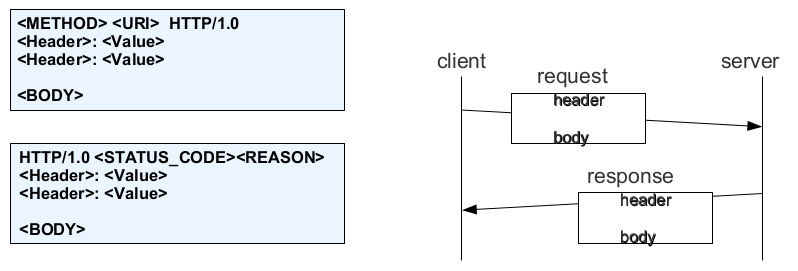
\includegraphics[scale=0.43]{chapters/6/assets/schema_m.png}
            \end{center}

        \subsubsection{Metodi di richieste HTTP}
            Essi sono:
            \begin{itemize}
                \item \textbf{GET}: richiede tutte le informazioni disponibili per un determinato URL. Il body del messaggio non è utilizzato.
                
                \verb:GET /index.html HTTP/1.0:

                \item \textbf{GET} condizionale: nel body viene inserita un'espressione del tipo:
                
                \verb:GET /index.html HTTP/1.0:\\
                \verb&If-Modified-Since: Wed, 19 Oct 2005 10:50:00 GMT&

                \item \textbf{HEAD}: richiede solo l'header, senza la risorsa (il file HTML, l'immagine, etc.), usato sopratutto per la diagnostica.
                
                \verb:HEAD /index.html HTTP/1.0:

                \item \textbf{POST}: è stato concepito in origine per inviare al server molte informazioni (nel body della richiesta), senza un limite sulle quantità di dati da trasmettere e sul tipo, ed in modo non visibile da URL.

                \verb:POST /prog.cgi HTTP/1.0:\\
                \verb=Content-length: 10=\\
                \verb:0123456789:

                \item \textbf{OPTIONS}: richiede l'elenco dei metodi permessi dal server.
                
                \verb:OPTIONS * HTTP/1.0:\\
                \verb:[riga vuota]:\\
                \verb:...:\\
                \verb-Allow: GET, HEAD, POST, OPTIONS, TRACE-

                \item \textbf{TRACE}: traccia una richiesta, visualizzando come viene trattata dal server.
                \item \textbf{DELETE}: cancella una risorsa (file) sul server. L'utente con cui gira il web server deve poter avere permessi in scrittura sul file indicato ed il server deve essere configurato per poterlo fare.
                \item \textbf{PUT}: upload di un file sul server con il nome indicato ed i contenuti specificati nel body.
            \end{itemize}

            La prima riga della risposta del server contiene un codice che classifica la risposta:
            \begin{table}[h]
                \centering
                \begin{tabular}{|c|l|l|}
                    \hline
                    \rowcolor[HTML]{000000} 
                    {\color[HTML]{EFEFEF} \textbf{Code}} & \multicolumn{1}{c|}{\cellcolor[HTML]{000000}{\color[HTML]{EFEFEF} \textbf{Meaning}}} & \multicolumn{1}{c|}{\cellcolor[HTML]{000000}{\color[HTML]{EFEFEF} \textbf{Examples}}} \\ \hline
                    1xx & Information & 100 = Server agrees to handle client's request \\ \hline
                    2xx & Success & 200 = Request succeded, 204 = No content present \\ \hline
                    3xx & Redirection & 301 = Page moved, 304 = Cached page still valid \\ \hline
                    4xx & Client error & 403 = Forbidden page, 404 = Page not found \\ \hline
                    5xx & Server error & 500 = Internal server error, 503 = Try again later \\ \hline
                \end{tabular}
            \end{table}

            \begin{center}
                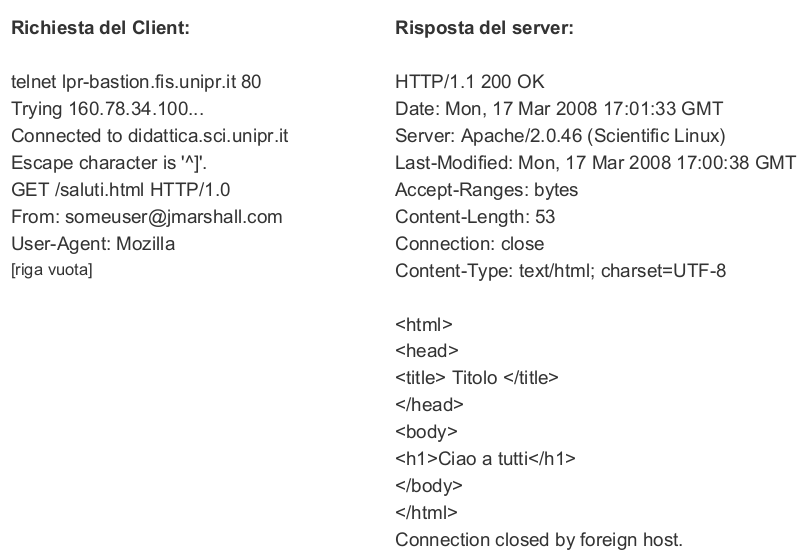
\includegraphics[scale=0.4]{chapters/6/assets/schema_n.png}
            \end{center}

        \subsubsection{HTTP 1.1: connessioni persistenti e parallele}
            HTTP 1.0 richiede la connessioni TCP tra due richieste successive.
            HTTP 1.1 supporta connessioni persistenti (riutilizzo di una connessione per diverse richieste).
            HTTP 1.1 supporta anche le richieste parallele.

            \begin{center}
                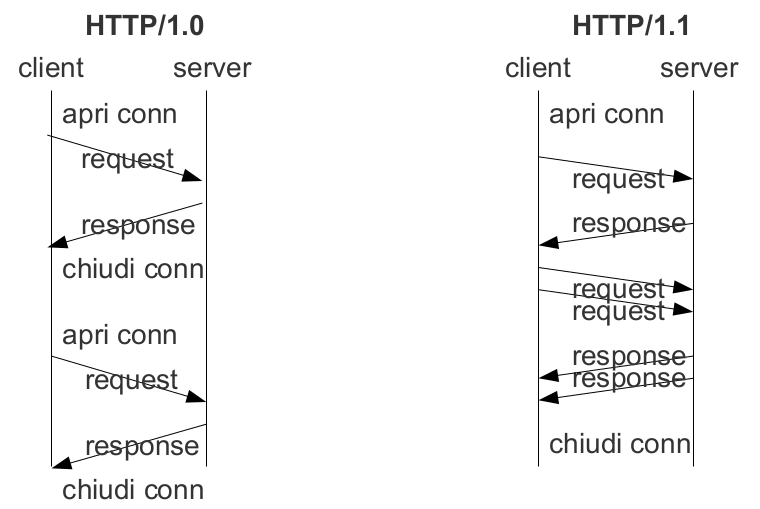
\includegraphics[scale=0.4]{chapters/6/assets/schema_o.png}
            \end{center}

        \subsubsection{HTTP 1.1: Chunked Transfering Encoding}
            In HTTP 1.0 chi spedisce un dato include nell'intestazione la dimensione in byte del dato stesso, mediante l'intestazione \verb-Content-length: nn-.
        
            \textbf{Chunked Transfere Encoding} è una modalità di trasferimento introdotta in HTTP 1.1 in cui i dati vendono inviati in una serie di \textbf{chunk}. Viene utilizzata per la trasmissione di dati generati dinamicamente, di cui non conosciamo la lunghezza prima di iniziare la trasmissione.
        
            Si utilizza \verb=Transfer-Encoding: chunked= invece di \verb-Content-length: xx-.\\
            La dimensione di ogni chunk viene inviata appena prima del chunk stesso in modo che il ricevente possa capire quando ha finito di ricevere il chunk. Il trasferimento termina con un chunk finale pari a 0.
            
            \verbatiminput{chapters/6/assets/schema_p.txt}

        \subsubsection{Pagine web statiche e dinamiche}
            Le pagine statiche sono file sul disco del server che vengono spediti al client assieme ad una intestazione (content-type, etc.).
        
            Nelle \textbf{pagine dinamiche} il documento viene generato in tempo reale, su richiesta. La generazione è eseguita da un programma che può essere eseguito:
            \begin{itemize}
                \item \textbf{dal server}: via CGI (programmi esterni richiamati dal server); oppure tramite scripting PHP, JSP, ASP.
                \item \textbf{dal client}: tramite Javascript, Java Applet (richiede JVM sul client), ActiveX (tecnologia Microsoft, codice compilato per Intel).
            \end{itemize}

            \begin{center}
                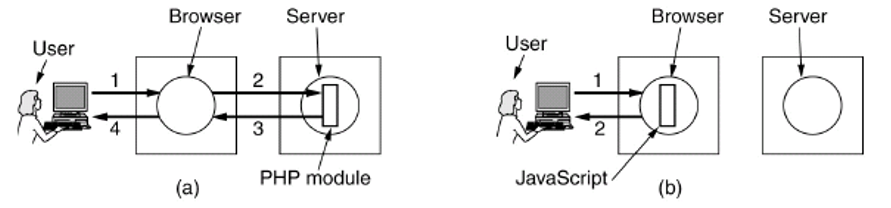
\includegraphics[scale=0.38]{chapters/6/assets/schema_q.png}
            \end{center}

        \subsubsection{Pagine dinamiche con CGI}
            Il protocollo \textbf{CGI (Common Gateway Interface)} consente di mettere in esecuzione un programma eseguibile sul server e di redirigere lo standard output del programma verso il client, il quale lo interpreterà come una normale risposta HTTP.
        
            Per attivare un programma il client utilizza la stesso modello URI utilizzato per il riferimento alle pagine statiche, con i metodi GET o POST.
        
            Il server può riconoscere un programma CGI in base alla sua estensione (\verb:.cgi:) o alla sua posizione (es. \verb:/cgi-bin/...:).
        
            Normalmente l'output è in formato HTML, ma può assumere anche altre forme (immagini, dati binari, istruzioni particolari per il browser, etc.).

            \begin{center}
                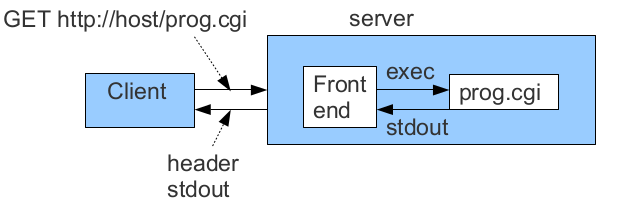
\includegraphics[scale=0.4]{chapters/6/assets/schema_r.png}
            \end{center}

        \subsubsection{Passaggio dei parametri}
            L'esecuzione di una pagina dinamica deve prevedere la possibilità di passare parametri o dati all'eseguibile.
        
            Questo può avvenire con due metodi alternativi: GET e POST:
            \begin{itemize}
                \item \textbf{il metodo GET} codifica i parametri della stringa URL.
                \item \textbf{il metodo POST} utilizza la parte body della richiesta.
            \end{itemize}

            L'HTML fornisce diversi tag per la codifica di parametri nella forma NOME = valore, da passare con GET o POST.

            Ad esempio:

            \lstinputlisting[language=HTML]{chapters/6/assets/schema_s.html}

            \begin{center}
                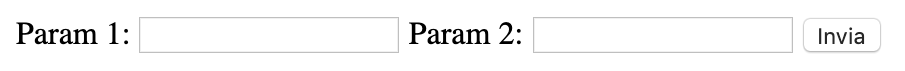
\includegraphics[scale=0.65]{chapters/6/assets/schema_t.png}

                Genera la URL: \verb-http://host/prog.cgi?param1=val1&param2=val2-
            \end{center}

        \subsubsection{Passaggio di dati con il metodo GET}
            Con il metodo GET la strinda di query (input) è in serita in coda alla URI del documento, preceduta dal carattere '?'.
        
            Ad esempio:\\
            \verb-GET http://host/prog.cgi?param1=val1&param2=val2 HTTP/1.0-\\
            \verb:header...:\\
            \verb:header...:\\
            \verb:<cr><lf>:

            Il programma riceve la stringa attraverso la variabile di ambiente \textbf{QUERY\_STRING}: \verb:QUERY\_STRING="param1=val1&param2=val2":

        \subsubsection{Passaggio di dati con il metodo POST}
            I parametri passati con il metodo POST vengono inseriti nel body della richiesta HTTP, ed il programma li riceve attraverso lo Standard Input.
        
            Ad esempio, se scegliamo il metodo POST nella FORM dell'esempio precedente:

            \verb-<form action=”http://host/prog.cgi” method=POST>-

            Otteniamo una richiesta HTTP del tipo:

            \verb-POST http://host/prog.cgi HTTP/1.0-

            \verb:header...:

            \verb=Content-length: 23=

            \verb:<cr> <lf>:

            \verb:param1=val1&param2=val2:

            Questo metodo ha due vantaggi nel passaggio dei parametri rispetto al metodo GET:
            \begin{itemize}
                \item i parametri non compaiono nella URI (e quindi non vengono tracciati nei file di log).
                \item è possibile trasferire non solo parametri, ma anche dati.
            \end{itemize}

        \subsubsection{Codifica e decodifica dei parametri}
            I parametri sono codificati dalla FORM in una unica stringa del tipo:

            \verb-http://host/prog.cgi?param1=val1&param2=val2-

            È compito del programma fare il parsing della stringa. La codifica utilizza diversi caratteri speciali (come = ? \&). Se i caratteri speciali compaiono all'interno dei parametri devono essere sostituiti.

            Lo spazio è sostituito con il carattere '+', mentre i caratteri speciali con la loro codifica ASCII preceduta dal carattere '\%'.

            Principali sostituzioni:
            \begin{center}
                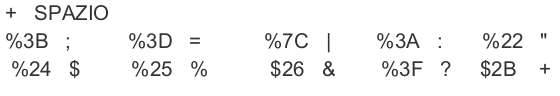
\includegraphics[scale=0.4]{chapters/6/assets/schema_u.png}
            \end{center}

        \subsubsection{Pagine dinamiche lato server: PHP}
            I server web supportano anche la possibilità di incorporare piccoli script all'interno del codice HTML, che verrà eseguito al momento della consultazione della pagina.
        
            Questo consente di realizzare documenti in cui solo una parte è dinamica.
        
            Un linguaggio molto utilizzato per questo scopo è il PHP. Ad esempio:

            \begin{center}
                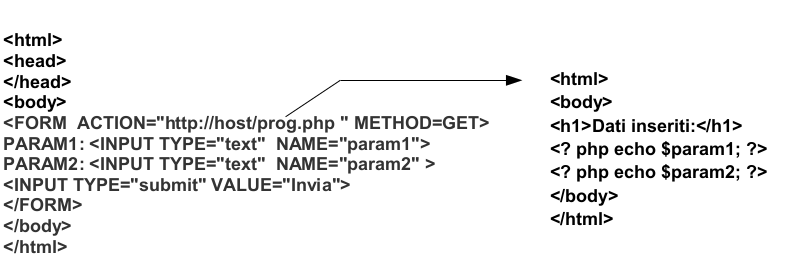
\includegraphics[scale=0.4]{chapters/6/assets/schema_v}
            \end{center}

        \subsubsection{Pagine dinamiche lato client: JavaScript}
            In altre applicazione è utile che il codice venga eseguito lato client. Anche il questo caso viene incorporato codice di script nella pagina HTML. Il linguaggio più popolare lato client è \textbf{JavaScript}.
        
            Ad esempio:
            \lstinputlisting[language=HTML]{chapters/6/assets/schema_w.html}

        \subsubsection{Pagine dinamiche lato client: Applet}
            Un altro metodo molto utilizzato è l'utilizzo di \textbf{Applet Java}.
        
            È necessario che il browser includa una JVM (ad oggi quasi nessuno per default). Le applet sono più portabili perché la JVM è la stessa su diverse piattaforme, mentre il supporto JavaScript può differire da una browser all'altro.
        
            Le applet possono essere incorporate nelle pagine HTML: \verb:<applet> ...: \verb:</applet>:. Ad esempio:

            \begin{center}
                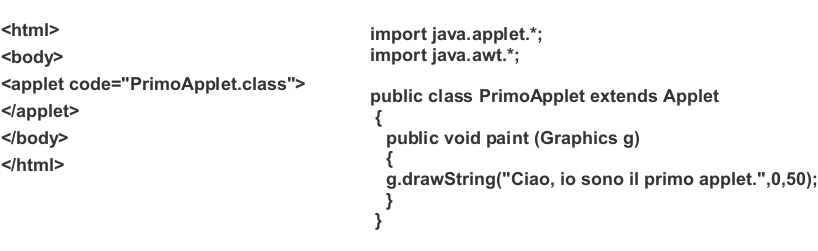
\includegraphics[scale=0.4]{chapters/6/assets/schema_x.png}
            \end{center}

        \subsubsection{Mancanza di stato e cookie}
            Il web è privo di stato: se un browser richiede più documenti da un server, ogni richiesta è indipendente; il server non ricorda più i contatti precedenti. In alcuni casi sarebbe utili avere memoria delle richieste, ad esempio, se l'accesso ai documenti richiede autenticazione, autorizzazione, etc.
        
            I \textbf{cookie} sono stati introdotti da \textbf{Netscape} per risolvere questo problema. I \textit{cookie} sono generati dal server, e scaricati assieme al documento. Il browser li memorizza in opportune directory, ma volendo, li può disabilitare. Informazioni contenute in un \textit{cookie}:

            \begin{table}[ht]
                \centering
                \begin{tabular}{|l|c|l|l|l|}
                    \hline
                    \rowcolor[HTML]{000000} 
                    \multicolumn{1}{|c|}{\cellcolor[HTML]{000000}{\color[HTML]{EFEFEF} \textbf{Domain}}} & {\color[HTML]{EFEFEF} \textbf{Path}} & \multicolumn{1}{c|}{\cellcolor[HTML]{000000}{\color[HTML]{EFEFEF} \textbf{Content}}} & \multicolumn{1}{c|}{\cellcolor[HTML]{000000}{\color[HTML]{EFEFEF} \textbf{Expires}}} & \multicolumn{1}{c|}{\cellcolor[HTML]{000000}{\color[HTML]{EFEFEF} \textbf{Sec}}} \\ \hline
                    toms-cap.com & / & CustomerID=497793521 & 15-10-02 17:00 & Yes \\ \hline
                    joes-store.com & / & Cart=1-00501;1-07031 & 11-10-02 14:22 & No \\ \hline
                    aportal.com & / & Prefs=Stk:SUNW+ORCL & 31-12-10 23:59 & No \\ \hline
                    sneaky.com & / & UserID=3627239101 & 31-12-10 23:59 & No \\ \hline
                \end{tabular}
            \end{table}


        \subsubsection{Contenuto dei cookie}
            \textbf{Contenuto} (nome/valore) è una variabile ed un campo obbligatorio.
        
            \textbf{Expire} (scadenza) è un attributo opzionale che permette di stabilire la data di scadenza del cookie. Può essere espressa come data, come numero massimo di giorni, oppure come now (adesso) (implica che il cookie venga eliminato subito dal computer dell'utente, in quanto scade nel momento in cui viene creato) o never (mai) (implica che il cookie non è soggetto a scadenza e questi sono denominati persistenti).
        
            \textbf{Dominio} e \textbf{Percorso} definiscono l'ambito di visibilità del cookie, indicano al browser che il cookie può essere inviato al server solo per il dominio ed il percorso indicati. Se non specificati, come predefiniti prendono il valore del dominio e del percorso che li ha inizialmente richiesti.
        
            \textbf{Secure} (Sicuro) indica se il cookie debba essere trasmesso criptato con HTTPS.

        \subsubsection{Come funzionano i cookie}
            Quando l'utente specifica un URL, il browser cerca tra i cookie che ha memorizzato un cookie (non scaduto) con lo stesso dominio dell'URL. Se esiste viene fatto upload del cookie nell'header assieme alla richiesta:
        
            \begin{center}
                \verb-Cookie: nome1=valore1;nome2=valore2-
            \end{center}
        
            La prima volta che viene richiesto un URL, nessun cookie verrà inviato dal browser, il server ne manderà uno assieme al documento:
        
            \verb|Set-Cookie: tuocodice=123; expires=Tue, 18-Mar-08 18:43:09 GMT|
            
            \verb|Set-Cookie: tuonome=Mario; expires=Tue, 18-Mar-08 18:43:09 GMT|

            Successive visite della stessa pagina saranno accompagnate dal cookie memorizzato che il server potrà aggiornare con la risposta. In questo modo il server memorizza le diverse visite del client.
        
        \subsubsection{Web Mobile}
            L'utilizzo del web da dispositivi mobili è in forte crescita. Presenta i seguenti problemi tecnici:
            \begin{itemize}
                \item Schermi piccoli.
                \item Difficile digitare URL lunghe.
                \item La banda può essere limitata.
                \item Connettività intermittente.
                \item Potenza di elaborazione limitata.
            \end{itemize}

            Possibili soluzioni per risolvere questo problema: il server determina il tipo di browser (campo User Agent) e genera formati adatti.

    \subsection{Web Services}
        I \textbf{web services} sono uno strumento innovativo per costruire middleware utilizzando componenti standard e aperti come XML per la codifica dei dati e HTTP, HTTPS o SMTP per il trasporto.

        Attraverso i \textit{web services} le applicazioni possono dialogare tra loro mediante un modello di interazione a chiamata di procedura remota.
    
        Implementazioni:
        \begin{itemize}
            \item \textbf{XML-RPC}: è la modalità più semplice, che implementa RPC. I messaggi sono codificati in XML e trasportati da HTTP.
            \item \textbf{SOAP}: sono realizzati mediante un'architettura (basata su HTTP) che stabilisce protocolli e componenti specifici.
            \item \textbf{REST}: i web services sono implementati come risorse WWW, quindi richiedono particolari architetture.
        \end{itemize}

        \begin{center}
            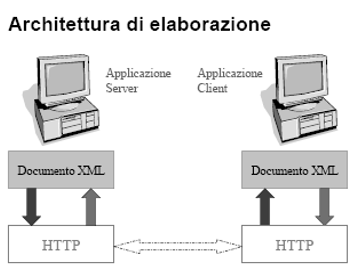
\includegraphics[scale=0.6]{chapters/6/assets/schema_y.png}
        \end{center}

        \subsubsection{Web Service: XML-RPC}
            È una specifica creata nel 1998 da UserLand Software. Da questo progetto è poi evoluta la specifica SOAP, anche se XML-RPC è ancora utilizzato per la sua semplicità.
        
            Le chiamate e le risposte sono codificate in XML e trasportate all'interno del body di HTTP. Le chiamate sono bloccanti.
        
            Esistono implementazioni per i principali linguaggi moderni (C/C++, Java, PHP, Python, etc.).
        
            L'interfaccia è indipendente dal linguaggio di programmazione e supporta un sottoinsieme dei tipi di dati semplici e composti:
            \begin{itemize}
                \item string (stringhe ASCII)
                \item int (con segno a 32 bit)
                \item double (float a 64 bit)
                \item boolean
                \item dateTime.iso8601 (orario nello standard ISO)
                \item base64 (dati binari codificati in ASCII con base64)
                \item array
                \item struct
            \end{itemize}

        \subsubsection{Web Service: SOAP}
            SOAP è l'architettura logico-funzionale, che permette l'interazione fra tre entità: Service Provider, Service Requester e Service Registry (Broker).

            I componenti di SOAP sono:
            \begin{itemize}
                \item SOAP: protocollo di interazione tra gli oggetti
                \item WDSL: linguaggio per descrivere gli oggetti (servizi web)
                \item UDDI: name \& service directory.
            \end{itemize}

            \begin{center}
                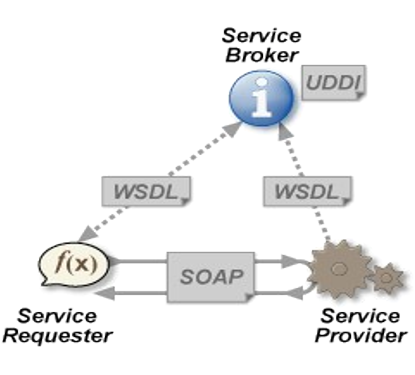
\includegraphics[scale=0.5]{chapters/6/assets/schema_z.png}
            \end{center}

    \subsection{Multimedia}
        Esistono diverse modalità di utilizzo del multimedia in internet, con diversi requisiti di rete:
        \begin{itemize}
            \item Streaming di contenuti registrati (Youtube). \item Realtime streaming (dirette SkyGo).
            \item Conferenze in tempo reale (Skype).
        \end{itemize}

        Questi utilizzi dipendono in vario modo dai seguenti fattori:
        \begin{itemize}
            \item Parametri della rete: throughput, latenza, jitter.
            \item Buffer del ricevente.
            \item Protocolli per l'invio del flusso multimediale (RTP).
            \item Protocolli di servizio per l'apertura, la gestione, e la chiusura della comunicazione.
        \end{itemize}

        \subsubsection{Streaming di contenuti registrati}
            Il modo più diretto per ascoltare musica è quello di usare il sistema classe di MIME e delle helpers applications: è un sistema popo efficiente perché si deve scaricare il file prima di iniziare l'ascolto.

            \begin{center}
                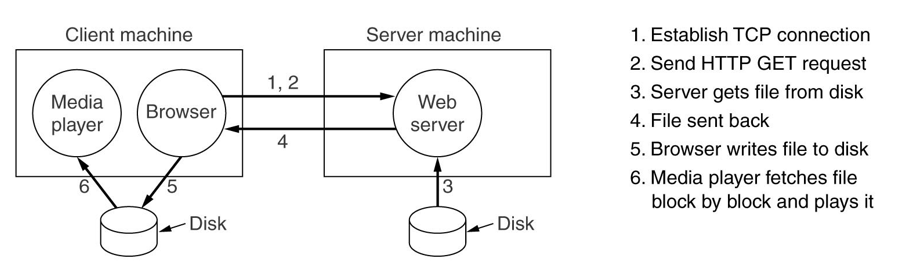
\includegraphics[scale=0.36]{chapters/6/assets/schema_za.png}
            \end{center}

        \subsubsection{Streaming con RTSP e RTP}
            La soluzione generalmente adottata (Audio Streaming) è la seguente : il file collegato al titolo non è quello contenente l'audio, ma un metafile che rimanda al file vero e proprio audio da ascoltare (il contenuto potrebbe essere la sola riga \verb|rtsp://server/file.mp3|).
        
            Il browser, una volta passato il metafile all'applicazione esterna, non fa più parte del ciclo di comunicazione.

            L'accesso al file multimediale (es. \verb|rtsp://server/file.mp3|) avviene mediante un protocollo per la gestione dell'interfaccia utente (Play/Record/Pause/etc.) denominato \textbf{RTSP (Real Time Streaming Protocol)}.

            \begin{center}
                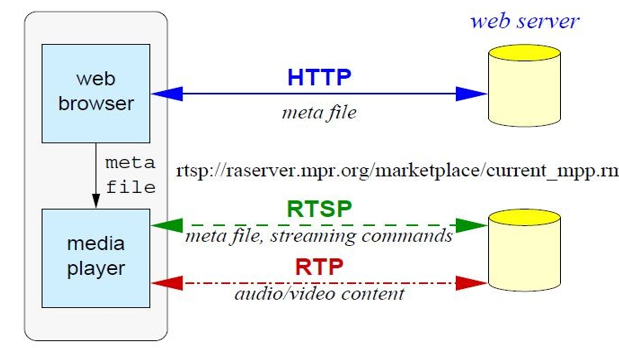
\includegraphics[scale=0.5]{chapters/6/assets/schema_zb.png}
            \end{center}

            Il protocollo supporta un set di comandi che vengono inviati al server mediante uno scambio testuale (simile all'HTTP):

            \begin{table}[h]
                \centering
                \begin{tabular}{|l|l|}
                    \hline
                    \rowcolor[HTML]{000000} 
                    \multicolumn{1}{|c|}{\cellcolor[HTML]{000000}{\color[HTML]{EFEFEF} \textbf{Command}}} & \multicolumn{1}{c|}{\cellcolor[HTML]{000000}{\color[HTML]{EFEFEF} \textbf{Server action}}} \\ \hline
                    DESCRIBE & List media parameters \\ \hline
                    SETUP & Establish a client-server logical channel \\ \hline
                    PLAY & Start sending data to the client \\ \hline
                    RECORD & Start accepting data from the client \\ \hline
                    PAUSE & Temporarily stop sending data \\ \hline
                    TEARDOWN & Release the logical channel \\ \hline
                \end{tabular}
            \end{table}

            YouTube usa HTTP/TCP. RTSP è comunque utilizzata per per la rete dei cellulari. I video sono memorizzati nella CDN di Google.

            RTSP è un protocollo di controllo e non si occupa della consegna dei dati, per questo viene spesso utilizzato assieme ad un protocollo specifico per il trasferimento dei dati, come il \textbf{RTP (Real-Time Transport Protocol)}.

            RTP è un protocollo è un protocollo client/server per il trasporto di flussi anche multipli di dati audio e video. È basato su UDP e può funzionare sia in unicast che in multicast.

            I campi principali dell'intestazione RTP sono:
            \begin{itemize}
                \item \textbf{Payload type}: rende possibile l’identificazione del contenuto (es. 26 $\rightarrow$ JPEG, 32 $\rightarrow$ MPEG1, 33 $\rightarrow$ MPEG2).
                \item \textbf{Sequence Number}: numerazione progressiva per il riordino.
                \item \textbf{Timestamp}: istante di campionamento del primo byte nel payload.
                \item \textbf{Synchronized Source ID}: identificatore della sorgente di stream, per distinguere diversi flussi contemporanei.
            \end{itemize}

            Con l'aiuto di un piccolo buffer il ricevente può ricostruire il flusso nella sequenza temporale corretta e sincronizzare eventuali flussi contemporanei.

            \begin{center}
                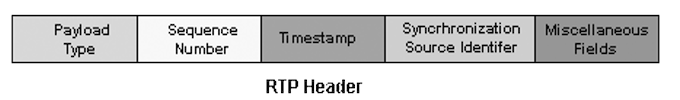
\includegraphics[scale=0.5]{chapters/6/assets/schema_zc.png}
            \end{center}

        \subsubsection{Realtime streaming}
            Su Internet sono sempre più diffusi prodotti audio/video in realtime. Principalmente emittenti radio e TV che trasmettono i programmi in internet parallelamente alle trasmissioni via etere.
        
            Rispetto ai contenuti registrati on-demand è necessario ridurre la bufferizzazione lato client per minimizzare lo scostamento temporale rispetto alla trasmissione via etere. Il ritardo è tipicamente di 10-15 secondi. Gli eventi streaming live vedono di solito centinaia o migliaia di utenti contemporanei, per cui la trasmissione "dovrebbe" usare il multicast e i protocolli RTP/UDP.
        
            Sorge un problema: sia multicasting che la porta RTP possono incontrare problemi nel supporto da parte dei provider. In molti casi viene usato Web streaming (HTTP/TCP) in unicast. Questo funziona bene se il numero di utenti è moderato. In questo caso è necessario mettere un server in un posto con buona connettività internet.

        \subsubsection{Conferenze in tempo reale}
            Principalmente avviene tramite \textbf{Voice over IP (VoIP)}:
            \begin{itemize}
                \item \textbf{Throughput}: la fonia ha limitate esigenze di thorughput (64Kbps, anche meno se compresso).
                
                \item \textbf{Latenza}: deve essere bassa, la rete telefonica considera accettabili latenze in una direzione entro 150 ms.
                
                Il ritardo di propagazione per 8000 Km (Seattle - Amsterdam) è di 40ms, a cui si aggiungono i ritardi introdotti dai router.
                
                Si aggiunge il ritardo dovuto al riempimento del pacchetto: un pacchetto da 1KB impiega 125ms per riempirsi a 64Kbps. Se si utilizzano pacchetti piccoli (160 bytes) è possibile ridurre la latenza, accettando un degrado di larghezza di banda.
                Altra latenza è data dal software (compressione / decompressione), soprattutto per i video.
                
                \item \textbf{Buffer}: è ancora necessario per evirare riproduzioni a scatti, ma deve essere piccolo per limitare la latenza. La presenza del buffer consente comunque la gestione dei pacchetti ricevuti fuori ordine mediante l'uso del numero di sequenza.
                
                \item \textbf{Protocolli}: occorre un protocollo per il trasporto dei dati, che generalmente è RTP/UDP. Il protocollo RTCP serve per lo scambio di messaggi di controllo, qualità del servizio, controllo di sessione, etc.
            \end{itemize}

        \subsubsection{VoIP con H323}
            H323 rappresenta una panoramica architetturale (dal punto di vista dell'industria telefonica) della telefonia Internet.
        
            Non emette proprie specifiche, ma fa riferimento a diversi protocolli specializzati: codifica del parlato, impostazione delle chiamate, segnalazione, trasporto di dati, etc.

            \begin{center}
                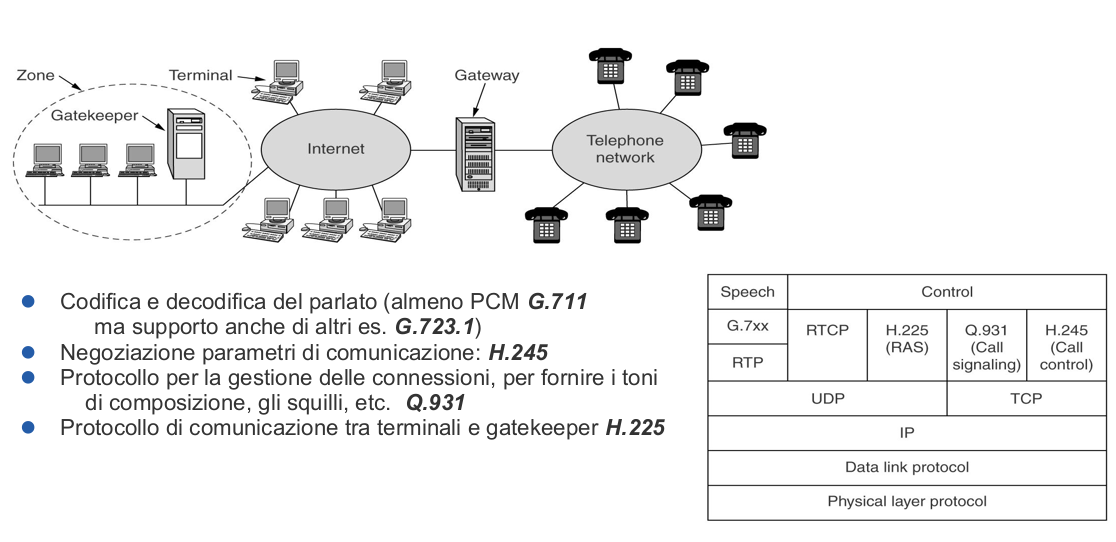
\includegraphics[scale=0.30]{chapters/6/assets/schema_zd.png}
            \end{center}

        \subsubsection{VoIP con SIP}
            \textbf{SIP (Session Initial Protocol)} è la riposta di IETF ad H323, considerato un prodotto tipico per telecomunicazioni (grande, complesso e poco flessibile), con un protocollo più semplice e modulare per la telefonia via Internet.
        
            Descrive come impostare le telefonate via internet, le videoconferenze e altre connessioni multimediali. Gestisce solamente l'impostazione, la gestione e la terminazione delle sessioni.
        
            Altri protocolli si occupano del trasporto dei dati. Per il traffico multimediale si usa di preferenza RTP.

        \subsubsection{Architettura SIP}
            I principali elementi dell'architettura SIP sono:
            \begin{itemize}
                \item \textbf{User Agent}: è un end-point e può fungere da client o server.
                \item \textbf{Proxy Server}: è un server intermedio, può rispondere direttamente alle richieste oppure inoltrarle ad un client, ad un server o ad un ulteriore proxy.
                Un proxy server analizza i parametri di instradamento dei messaggi e "nasconde" la reale posizione del destinatario del messaggio (essendo quest'ultimo indirizzabile con un nome convenzionale del dominio di appartenenza).
                \item \textbf{Location Server}: è un database contenente informazioni sull'utente, come il profilo, l'indirizzo IP, l'URL.
            \end{itemize}

            \begin{center}
                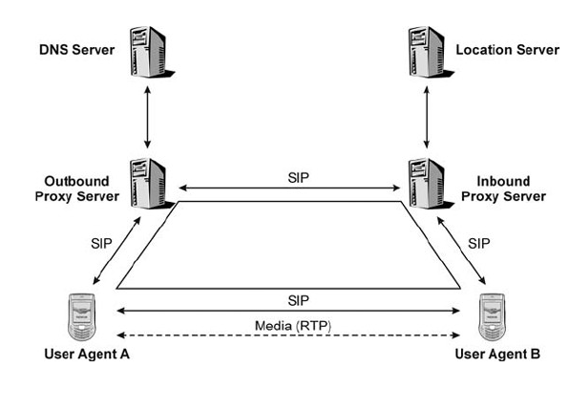
\includegraphics[scale=0.5]{chapters/6/assets/schema_ze.png}
            \end{center}

        \subsubsection{Il Protocollo SIP}
            Un \textbf{SIP-URI} rappresenta lo schema di indirizzamento SIP per chiamare un altro soggetto attraverso il protocollo SIP.
        
            In altre parole, un SIP URI è il recapito telefonico SIP di un utente. Il SIP URI assomiglia ad un indirizzo e-mail scritto nel seguente formato standard: \verb|{sip/sips}:[user-part@]domain-part[:port]|
        
            Esempio: \verb|sip:alfierir@ekiga.net|
        
            Queste URI possono contenere indirizzi IPv4, IPv6 o numeri di telefono veri e propri: \verb|sips:+004437612234@sip-proxy.org:5062|

            Il protocollo è basato su UDP/5060 con transazioni richiesta/risposta in ASCII (simile ad HTTP).

            Una transazione inizia con una \textbf{Request} inviata da uno User Agent Client ad un Proxy e termina con una \textbf{Final Response} inviata in senso inverso. L'RFC 3261 definisce i seguenti metodi:

            \begin{table}[h]
                \centering
                \begin{tabular}{|l|l|}
                    \hline
                    \rowcolor[HTML]{000000} 
                    \multicolumn{1}{|c|}{\cellcolor[HTML]{000000}{\color[HTML]{EFEFEF} \textbf{Method}}} & \multicolumn{1}{c|}{\cellcolor[HTML]{000000}{\color[HTML]{EFEFEF} \textbf{Description}}} \\ \hline
                    INVITE & Request initiation of a session \\ \hline
                    ACK & Confirm that a session has been initiated \\ \hline
                    BYE & Request termination of a session \\ \hline
                    OPTIONS & Query a host about its capabilities \\ \hline
                    CANCEL & Cancel a pending request \\ \hline
                    REGISTER & Inform a redirection server about client's current location \\ \hline
                \end{tabular}
            \end{table}

            \begin{center}
                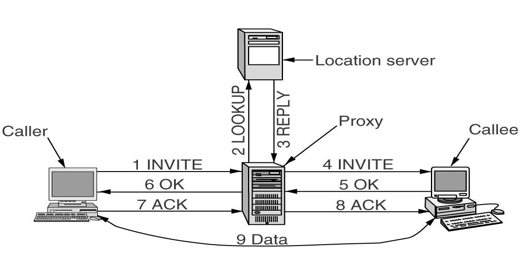
\includegraphics[scale=0.6]{chapters/6/assets/schema_zf.png}
            \end{center}